\section{Experiments}
\subsection{Experimental Settings}
\textbf{Implementation.} We finetune an 8B Qwen-3~\citep{yang2025qwen3} on TimeToolBench (Section~\ref{sec: timetoolbench}) with the proposed training strategy in Section~\ref{sec: training strategy}. During the training process, we adopt the LlamaFactory~\citep{zheng2024llamafactoryunifiedefficientfinetuning}, apply LoRA~\citep{hulora}, train the model with 8 NVIDIA 3090 GPUs. We then equip the trained Qwen-3 with TimeART for evaluation. For simplification, \textit{we denote our method as TimeART in the following parts.}

\textbf{Benchmarks.} We evaluate TimeART on two well-recognized benchmarks MTBench~\citep{chen2025mtbench} and TimeMQA~\citep{TimeMQA}. Since part of the TimeToolBench is also constructed on source data in MTBench or TimeMQA, we remove them from the training set to avoid data leakage. 

\textbf{Evaluation Metrics.} We follow the evaluation protocols in TimeMQA and MTBench. For forecasting tasks like temperature forecasting and financial indicator forecasting, we follow the practice in MTBench to report the point-wise error, i.e., Mean Square Error (MSE), Mean Absolute Error (MAE), and Mean Absolute Percentage Error (MAPE). For TSQA tasks, we mainly adopt accurate rate (Acc) as the metric. Note that there exists two kinds of accurate rates (3-way and 5-way) in MTBench and we follow their settings.

\textbf{Baselines.} We compare TimeART against multiple closed-source and open-source models. For closed-source models, we choose GPT-4o~\citep{hurst2024gpt}, Gemini-2.0~\citep{team2023gemini}, DeepSeek~\citep{liu2024deepseek}, Claude-Sonnet-3.5~\citep{TheC3} and Qwen3-max~\citep{yang2025qwen3}. For open-source models, we select DeepSeek-R1-7B, Llama3-8B, Mistral-7B, ChatTS-7B, and Qwen3-8B. 

\subsection{Main Results}


\begin{table*}[t]
    \centering
    \caption{Results on Forecasting tasks in MTBench. Lower MSE, MAE, MAPE, MACD (MSE), and BB (MSE) values indicate better performance. \first{Red}: the best, \second{Blue}: the second best. }
    \label{tab: time series forecasting}
     \resizebox{1\linewidth}{!}{
    \begin{tabular}{c|c|cc|cc|cc|cc|cc|cc}
    \toprule
        \multirow{3}{*}{Model} & \multirow{3}{*}{Type} & \multicolumn{4}{c|}{Stock Price Forecasting}  & \multicolumn{4}{c|}{Stock Indicator Forecasting} & \multicolumn{4}{c}{Temperature Forecasting}  \\ \cmidrule{3-14}
        ~ & ~ & \multicolumn{2}{c|}{7-day} & \multicolumn{2}{c|}{30-day} & \multicolumn{2}{c|}{7-day} & \multicolumn{2}{c|}{30-day} & \multicolumn{2}{c|}{7-day} & \multicolumn{2}{c}{14-day} \\ \cmidrule{3-14}
        ~ & ~ & MAE & MAPE & MAE & MAPE & MACD & BB & MACD & BB & MSE & MAE & MSE & MAE  \\ \midrule
        \rowcg
        GPT-4o & closed & 1.596  & 2.544  & 2.338  & 3.520  & 0.365  & \second{1.082}  & 0.897  & \second{2.068}  & 17.550  & \second{3.110}  & 40.430  & 4.490   \\ \midrule
        Gemini & closed & 1.628  & 3.513  & 2.432  & 3.268  & 0.384  & 1.153  & 0.975  & 2.248  & 24.310  & 3.670  & 29.470  & 4.030   \\ \midrule
        \rowcg
        Claude & closed & 1.422  & \second{2.098}  & 2.065  & \second{2.847}  & 0.373  & 1.246  & 1.171  & 2.345  & \second{4.110}  & 3.500  & 25.080  & 3.750   \\ \midrule
        DeepSeek & closed & 1.720  & 2.135  & 2.134  & 3.305  & \second{0.352}  & 1.187  & 1.072  & 2.201  & 29.380  & 4.040  & 101.280  & 6.610  \\ \midrule
        \rowcg
        DeepSeek-R1 7B & open & 1.137 & 4.846 & \second{1.304} & 4.669 & 0.871  & 2.045  & 1.526  & 2.762  & 28.039  & 4.214  & 32.732 & 4.491  \\ \midrule
        ChatTS 7B & open & \second{0.866}  & 2.925  & 1.339  & 3.071  & 2.047  & 2.014  & 3.342  & 2.364  & 19.512  & 3.407  & \second{23.750} & \second{3.742}  \\ \midrule
        \rowcg
        Qwen3 8B & open & 1.106  & 5.441  & 1.313  & 5.241  & 0.359 & 2.038  & \second{0.887}  & 2.940  & 24.144  & 3.841  & 49.084 & 5.474   \\ \midrule
        \rowcr
        \textbf{TimeART} & Open & \first{0.788}  & \first{1.634}  & \first{1.122}  & \first{3.054}  & \first{0.347}  & \first{1.032} & \first{0.862}  & \first{1.982}  & \first{4.021}  & \first{1.627}  & \first{5.026}  & \first{1.782}  \\ \bottomrule
    \end{tabular}}
\end{table*}


\begin{table*}[!htbp]
    \centering
    \caption{Results on Reasoning tasks in MTBench. Higher accuracy rates (Acc, 3-way, 5-way) indicate better performance. \first{Red}: the best, \second{Blue}: the second best. }
    \label{tab: time series reasoning}
    \resizebox{1\linewidth}{!}{
    \begin{tabular}{c|c|cc|cc|cc|cc|c|c|c|c}
    \toprule
        \multirow{3}{*}{Model} & \multirow{3}{*}{Type} & \multicolumn{4}{c|}{Stock Trend Classification} & \multicolumn{4}{c|}{News-stock Correlation} & \multicolumn{2}{c|}{\makecell{News-finance \\ MCQA}} & \multicolumn{2}{c}{\makecell{Temperature Trend \\Classification}}   \\ \cmidrule{3-14}
        ~ & ~ & \multicolumn{2}{c|}{7-day} & \multicolumn{2}{c|}{30-day} & \multicolumn{2}{c|}{7-day} & \multicolumn{2}{c|}{30-day} & 7-day & 30-day & Past & Future  \\ \cmidrule{3-14}
        ~ & ~ & 3-way & 5-way & 3-way & 5-way & 3-way & 5-way & 3-way & 5-way & Acc & Acc & Acc & Acc  \\ \midrule
        \rowcg
        GPT-4o & closed & 42.81  & 36.45  & 47.35  & 30.58  & 53.60  & 31.00  & 57.60  & 34.60  & 65.10  & 52.80   & \second{66.36}  & 43.54   \\ \midrule
        Gemini & closed & \second{47.30}  & \second{41.50}  & 44.90  & 29.70  & 51.80  & 26.40  & \second{59.60}  & 34.80  & 63.60  & 50.30  & 56.96  & 51.76   \\ \midrule
        \rowcg
        Claude & closed & 44.90  & 33.40  & \second{52.05}  & 31.70  & 50.40  & 29.00  & 57.90  & 34.30  & 75.60  & 61.10    & 59.78  & \second{56.87}   \\ \midrule
        DeepSeek & closed & 45.12  & 35.60  & 48.26  & 29.55  & 50.00  & 27.10  & 57.50  & \second{35.00}  & 77.60  & 69.30  & 26.49  & 25.17   \\ \midrule
        \rowcg
        DeepSeek-R1 7B & open & 27.53  & 17.11  & 46.46  & 26.06  & 57.84 & 32.99 & 53.49 & 31.01 & \first{90.40} & \first{89.12} & - & -  \\ \midrule
        ChatTS 7B & open & 19.71  & 16.09  & 19.38  & 13.46  & 46.44 & 24.44 & 37.60 & 22.67 & 85.91 & \second{84.47} & 60.80  & 28.79   \\ \midrule
        \rowcg
        Qwen3 8B & open & 37.55  & 32.71  & 44.20  & \second{32.50}  & \second{58.66}  & \second{35.64}  & 51.16  & 28.49  & 69.25  & 58.20  & 38.23  & 17.10   \\ \midrule
        \rowcr
        \textbf{TimeART} & Open & \first{51.73}  & \first{45.07}  & \first{55.28}  & \first{41.25}  & \first{71.25}  & \first{42.36}  & \first{69.25}  & \first{40.52}  & \second{88.50}  & 78.50   & \first{76.22}  & \first{58.53}  \\ \bottomrule
    \end{tabular}}
\end{table*}
\textbf{Time Series Forecasting.} Table~\ref{tab: time series forecasting} presents time series forecasting results on stock and temperature data. Compared with conventional uni-modal forecasting, the tasks in Table~\ref{tab: time series forecasting} consider both the textual and temporal information with LLMs. For Stock Price Forecasting, the tasks are classified as short-term (7-day input, 1-day output) and long-term (30-day input, 7-day output), and we report the MSE and MAPE. For Stock Indicator Forecasting, we focus on the financial indicators Moving Average Convergence Divergence (MACD) and Uppder Band of the Bollinger Bands (BB)~\citep{chen2025mtbench}, and report the MSE. For Temperature Forecasting, we also follow the settings in MTBench to consider the short-term (7-day input, 1-day output) and long-term (14-day input, 3-day output) tasks, and report the MSE and MAE. 

Results demonstrate the state-of-the-art forecasting performance of TimeART. Compared with baselines, TimeART achieves large improvements in Stock Price Forecasting and Temperature Forecasting. Considering the MAE metric, TimeART achieves \textit{9\% -- 68\%} reduction across all settings. On Stock Indicator Forecasting tasks, we observe that LLMs can achieve good performance, which means these indicators are related to textual information. TimeART also achieves best accuracy because it adaptively integrates both the results from tools and the implicit information in texts.

\textbf{Time Series Reasoning.}
Table~\ref{tab: time series reasoning} and Table~\ref{tab: TimeMQA} present the results of Time Series Reasoning on MTBench and TimeMQA. In MTBench, the tasks include Stock Trend Classification, Temperature Trend Classification, News-stock Correlation and News-finance MCQA, which evaluate model's understanding and reasoning of domain texts and temporal correlations, and are organized into multiple-choice questions to calculate accuracy. For TimeMQA, we select the question-answer subsets, and classify them into four categories: Understanding, Perception, Reasoning, and Estimation. Similar to MTBench, they are also organized as multi-choise questions, so that we also report the accuracy. The details are introduced in Appendix~\ref{app: settings}.

\begin{table}[!htbp]
    \centering
    \caption{Accuracy rates on tasks in TimeMQA. Higher values indicate better performance. \first{Red}: the best, \second{Blue}: the second best. }
    \label{tab: TimeMQA}
    \resizebox{1\columnwidth}{!}{
    \begin{tabular}{c|c|c|c|c|c}
    \toprule
        \rowcb
        Model & Type & Understanding & Perception & Reasoning & Estimation \\ \midrule
        \rowcg
        \textit{GPT-4o} & \textit{closed} & 50.86  & 69.65  & 50.00  & 66.66  \\ \midrule     
        \textit{Qwen3-max} & \textit{closed} &53.45 &58.27 &46.25 &49.33  \\ \midrule   
        \rowcg
        DeepSeek-R1 7B & open  & 7.76  & 12.69  & 16.89  & 7.41  \\ \midrule
        
        Llama3 8B & open  & 33.62  & \second{36.27}  & 27.03  & 25.92  \\ \midrule
        \rowcg
        ChatTS 7B & open  & 25.00  & 28.68  & \second{38.51}  & 12.03  \\ \midrule
        Qwen3-8B & open  & \second{43.10}  & 35.20  & 36.80  & 25.00  \\ \midrule
        \rowcg
        \makecell{TimeMQA + \\ Llama3 8B} & open&28.45 &36.27 &22.97 &\second{40.74} \\ \midrule
        \makecell{TimeMQA + \\ Qwen2.5 7B} &open &10.34 &24.41 &13.51 &26.85 \\ \midrule
        \rowcg
        \makecell{TimeMQA + \\ Mistral 7B} & open  & 18.96  & 26.20  & 12.83  & 
        28.70  \\ \midrule
        \rowcr
        \textbf{TimeART} & open & \first{59.33}  & \first{62.34}  & \first{49.12}  & \first{57.41} \\ \bottomrule
    \end{tabular}}
\end{table}

Results show TimeART's strong capability on time series reasoning tasks. On each single task, TimeART outperforms all open-source baselines a lot, demonstrating the effectiveness of strategic tool-use. Compared with closed-source GPT-4o and Qwen3-max, TimeART also achieves competitive performance with much fewer parameters. We observe that DeepSeek-R1 7B seems to encounter financial data during the pre-training phase, where it performs decisively in financial reasoning tasks and achieves high accuracy rates--see Table~\ref{tab: time series reasoning}. However, it easily suffers over-thinking phenomena in other tasks, e.g, failure on Temperature Trend Classification, and poor performance on general reasoning tasks in Table~\ref{tab: TimeMQA}.

Overall, TimeART demonstrates excellent tool-use strategies in various tasks. For analytical tasks relying more on tools, TimeART can use corresponding tools to achieve strong performance. In reasoning tasks that the reasoning capability matters, TimeART does not show blind faith in tools; instead, it analyzes on the analytical results from them and draws reliable conclusions. We make furter model analyses in Section~\ref{sec: model analysis}.

\subsection{Model Analysis}
\label{sec: model analysis}

%timeart analysis: qwen3 qwen3+timeart trained qwen3+timeart qwen3max+timeart
\textbf{Ablations on the framework.} Since the proposed TimeART can be treated as a general tool-use framework for agentic time series reasoning, we further evaluate its effectivenss through designing some variants: 1) Original Qwen3 8B as a fundamental baseline; 2) Qwen3 8B with Tool-use. This variant incorporate original Qwen3 8B into TimeART, used to evaluate the improvements introduced by the TimeART framework; 3) Our proposed trained Qwen3 8B incorporated with TimeART; 4) Qwen3-max, used to evaluate the potential of closed-source LLMs; 5) Qwen3-max with Tool-use, used to further demonstrate the effectiveness of the TimeART framework. 

As shown in Figure~\ref{fig: ablations on framework}, we conduct experiments on the four categories of TSQA tasks from TimeMQA. We have following key observations: 1) Tool use is demonstrated important to time series reasoning tasks. Both the original Qwen3 8B and Qwen3-max can achieve direct improvements when equipped with the Tool-use in TimeART; 2) There seems to exist a cascading effect in TimeART's enhancement on LLMs, where stronger LLMs may achieve more improvements with Tool-use in TimeART. Experimental, the TimeART consistently improves the Qwen3-max more than Qwen3 8B  on all four tasks. This demonstrates the strong potential of TimeART as an agentic framework; 3) The proposed TimeToolBench is effective, and suitable for finetuning small-scale LLMs. The finetuned Qwen3 8B can acquire the strategic tool-use ability, thus achieving stronger performance than closed-source Qwen3-max with the help of TimeART.

\begin{figure}[t]
  \centering
  % 第一行
  \begin{minipage}[b]{0.49\linewidth}
    \centering
    \subfloat[Understanding.]
    {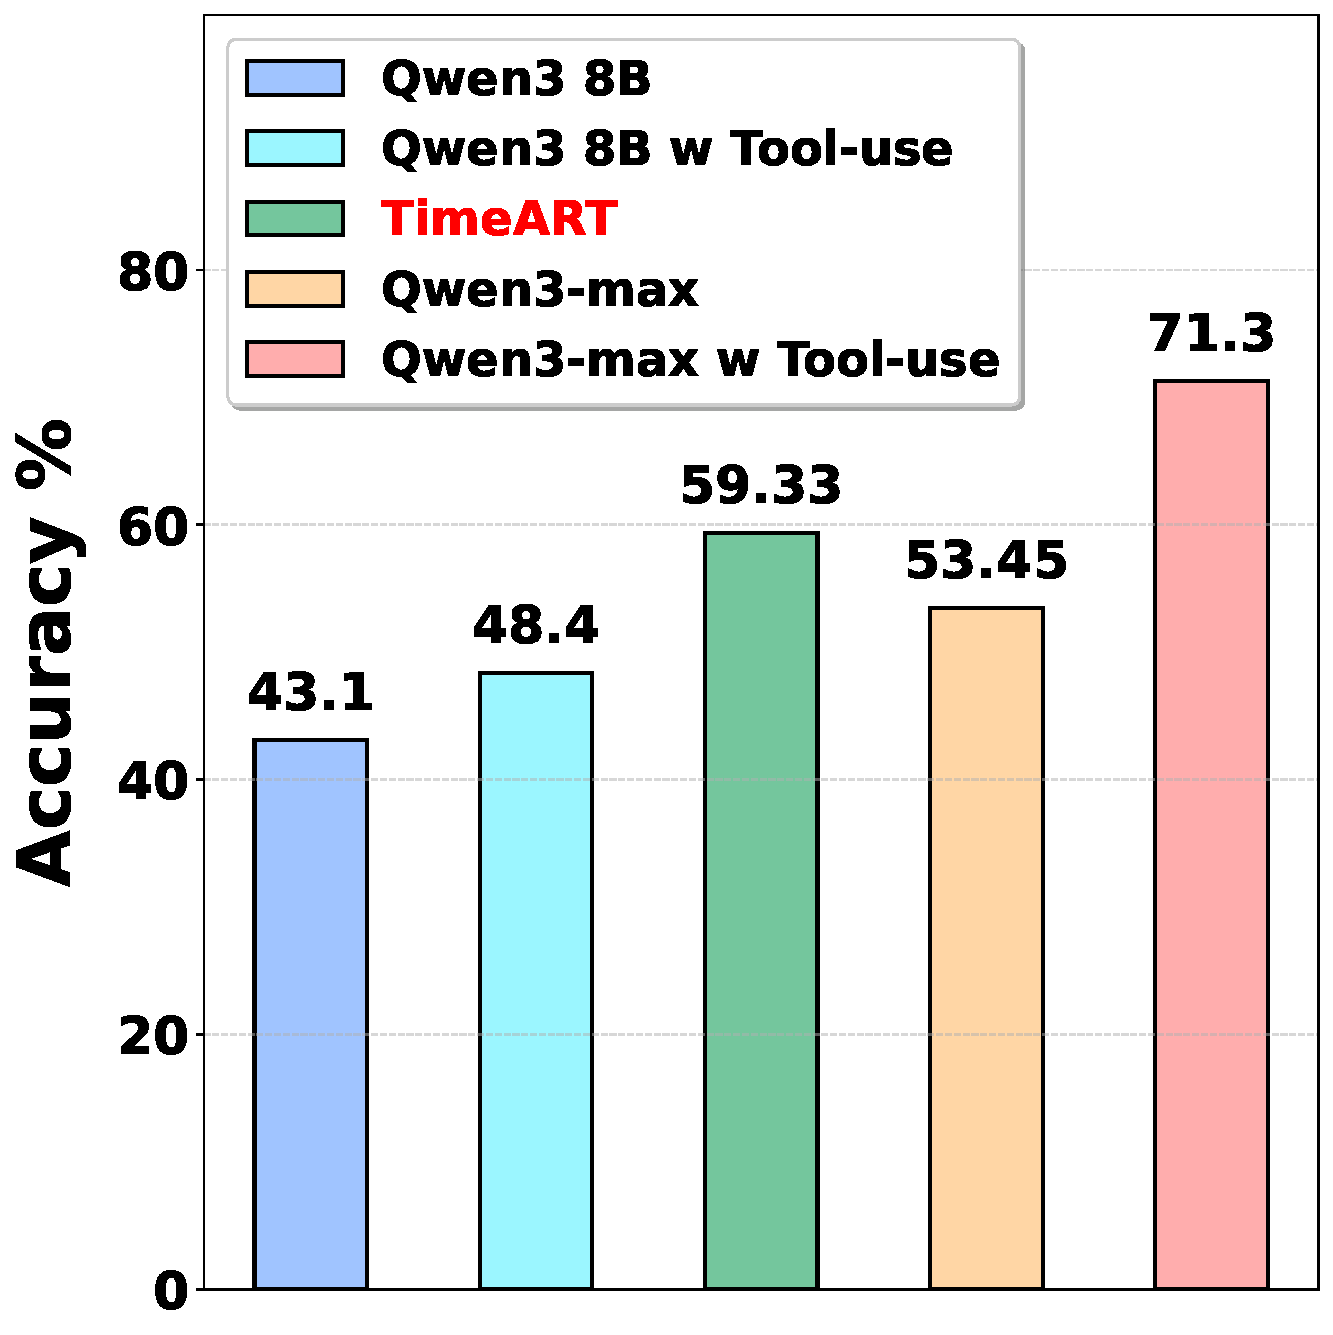
\includegraphics[width=\linewidth]{Figures/ablations-framework-understanding.pdf}}
  \end{minipage}
  \hfill
  \begin{minipage}[b]{0.49\linewidth}
    \centering
    \subfloat[Perception.]
    {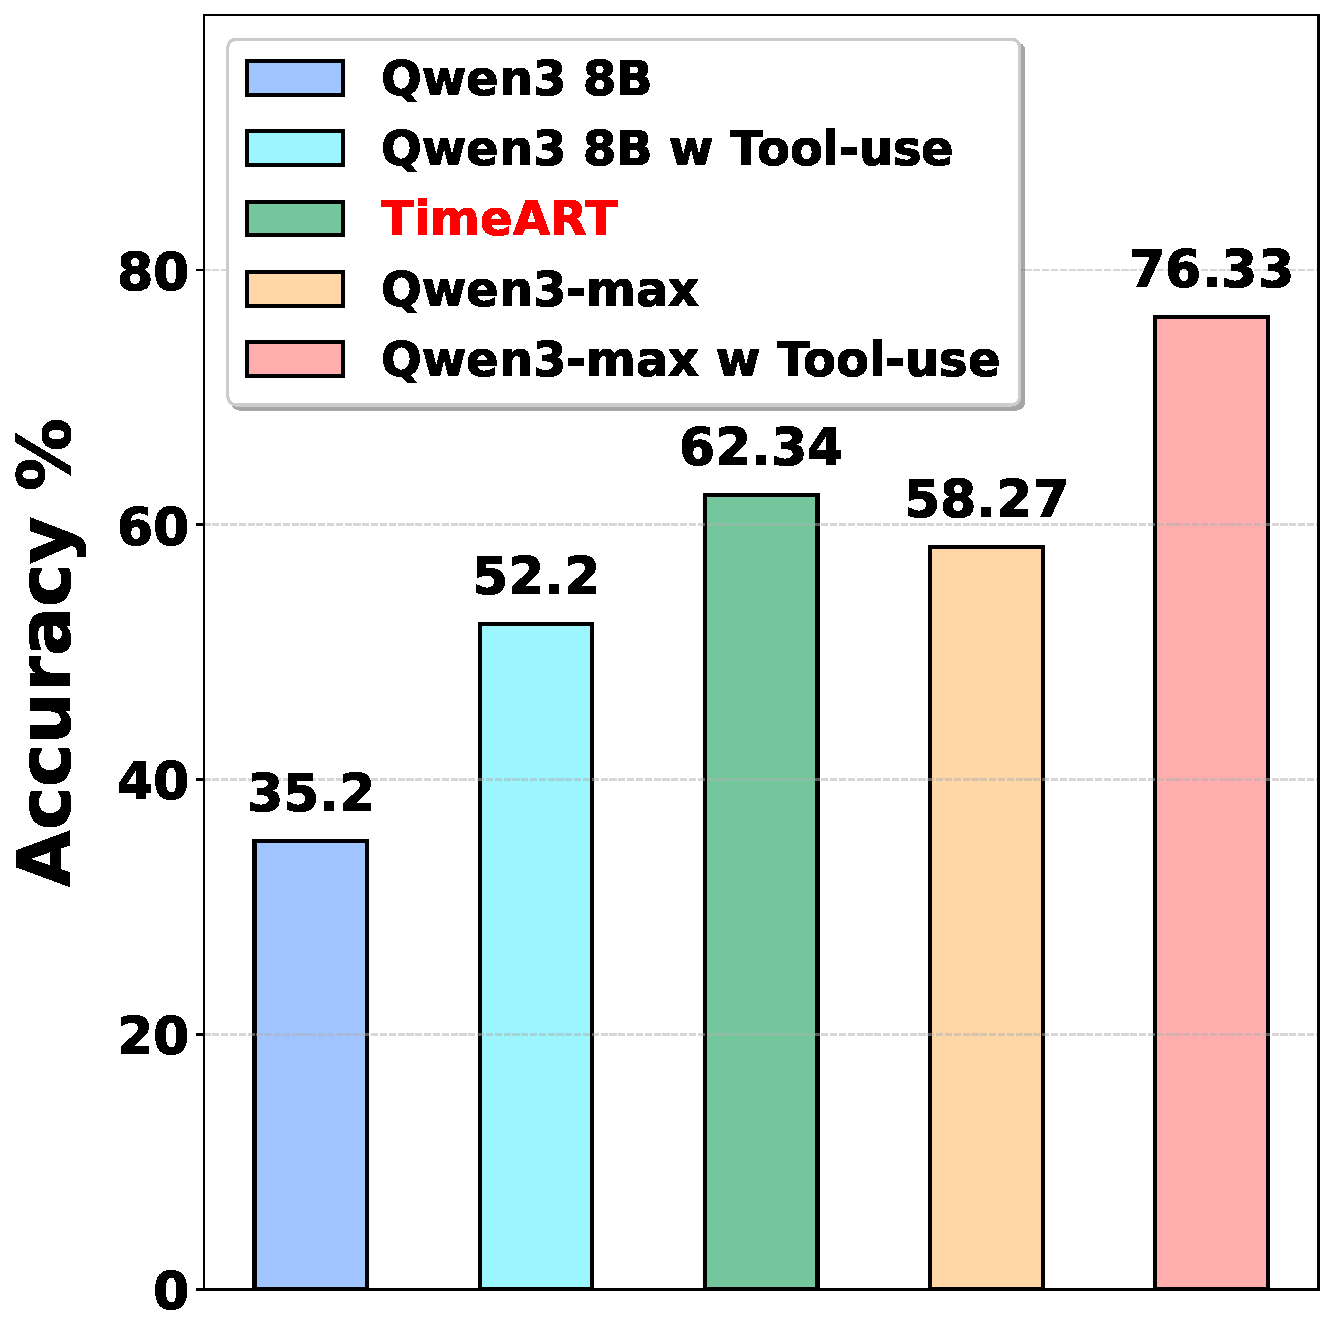
\includegraphics[width=\linewidth]{Figures/ablations-framework-perception.pdf}}
  \end{minipage}
  
  % 第二行
  \begin{minipage}[b]{0.49\linewidth}
    \centering
    \subfloat[Reasoning.]
    {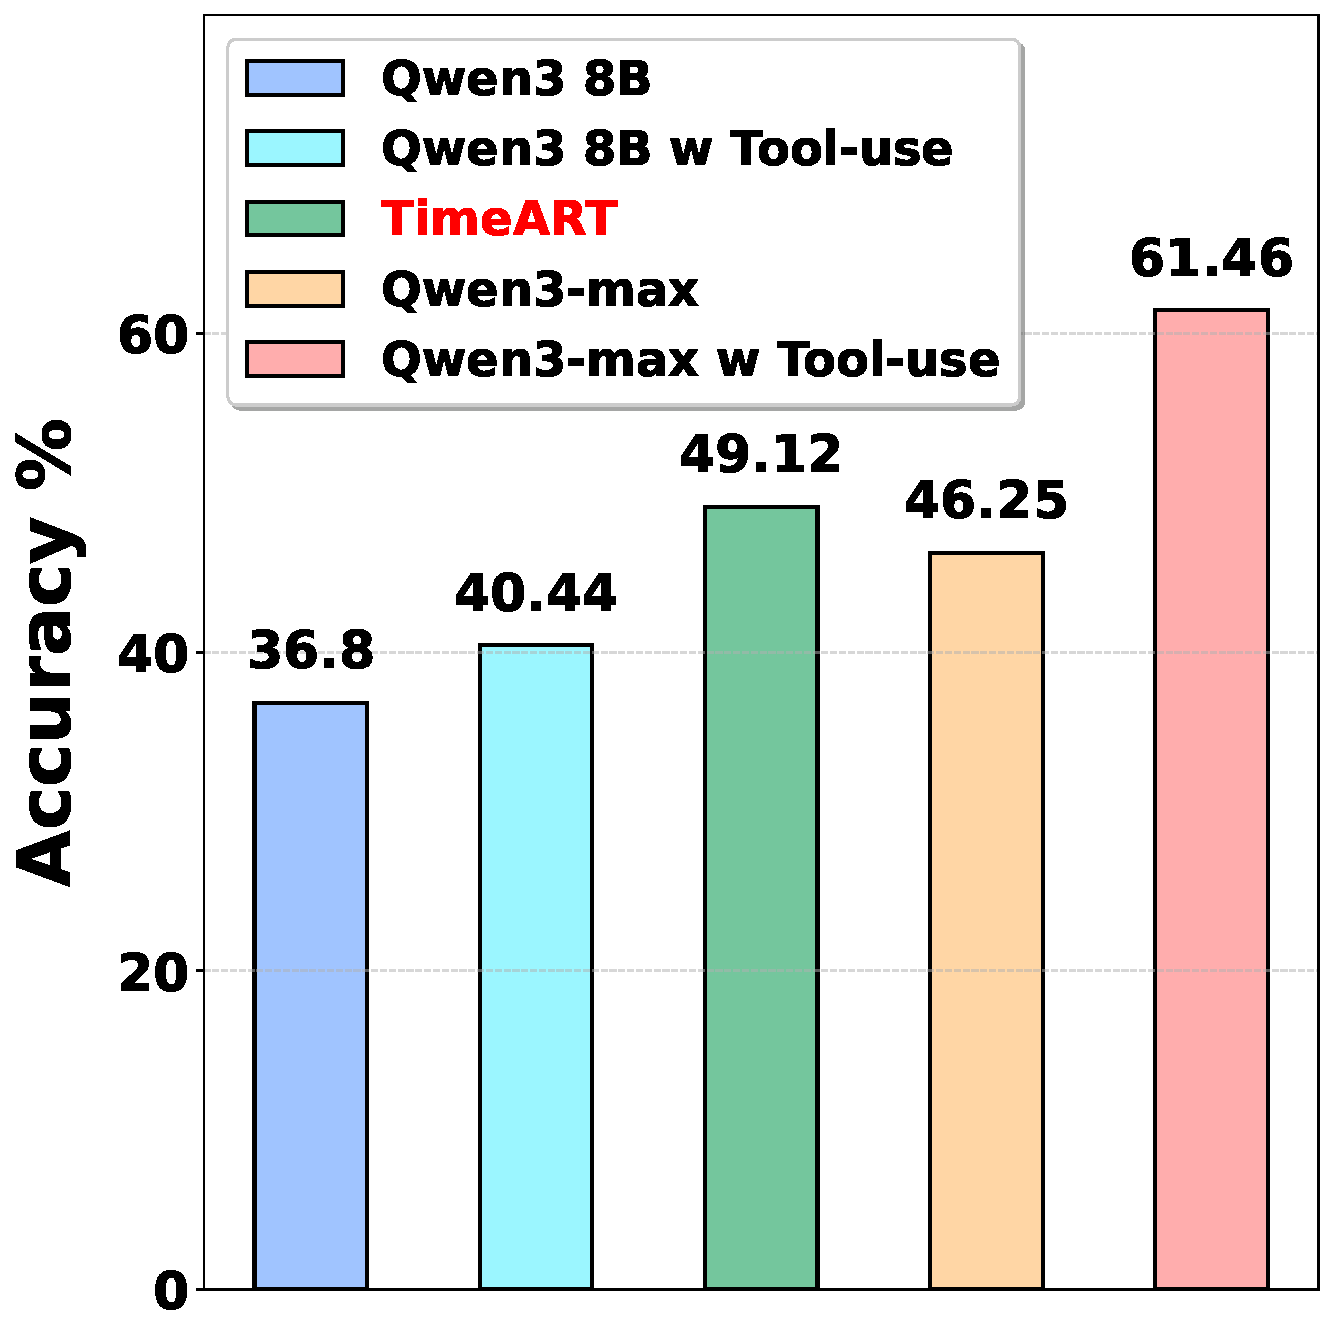
\includegraphics[width=\linewidth]{Figures/ablations-framework-reasoning.pdf}}
  \end{minipage}
  \hfill
  \begin{minipage}[b]{0.49\linewidth}
    \centering
    \subfloat[Estimation.]
    {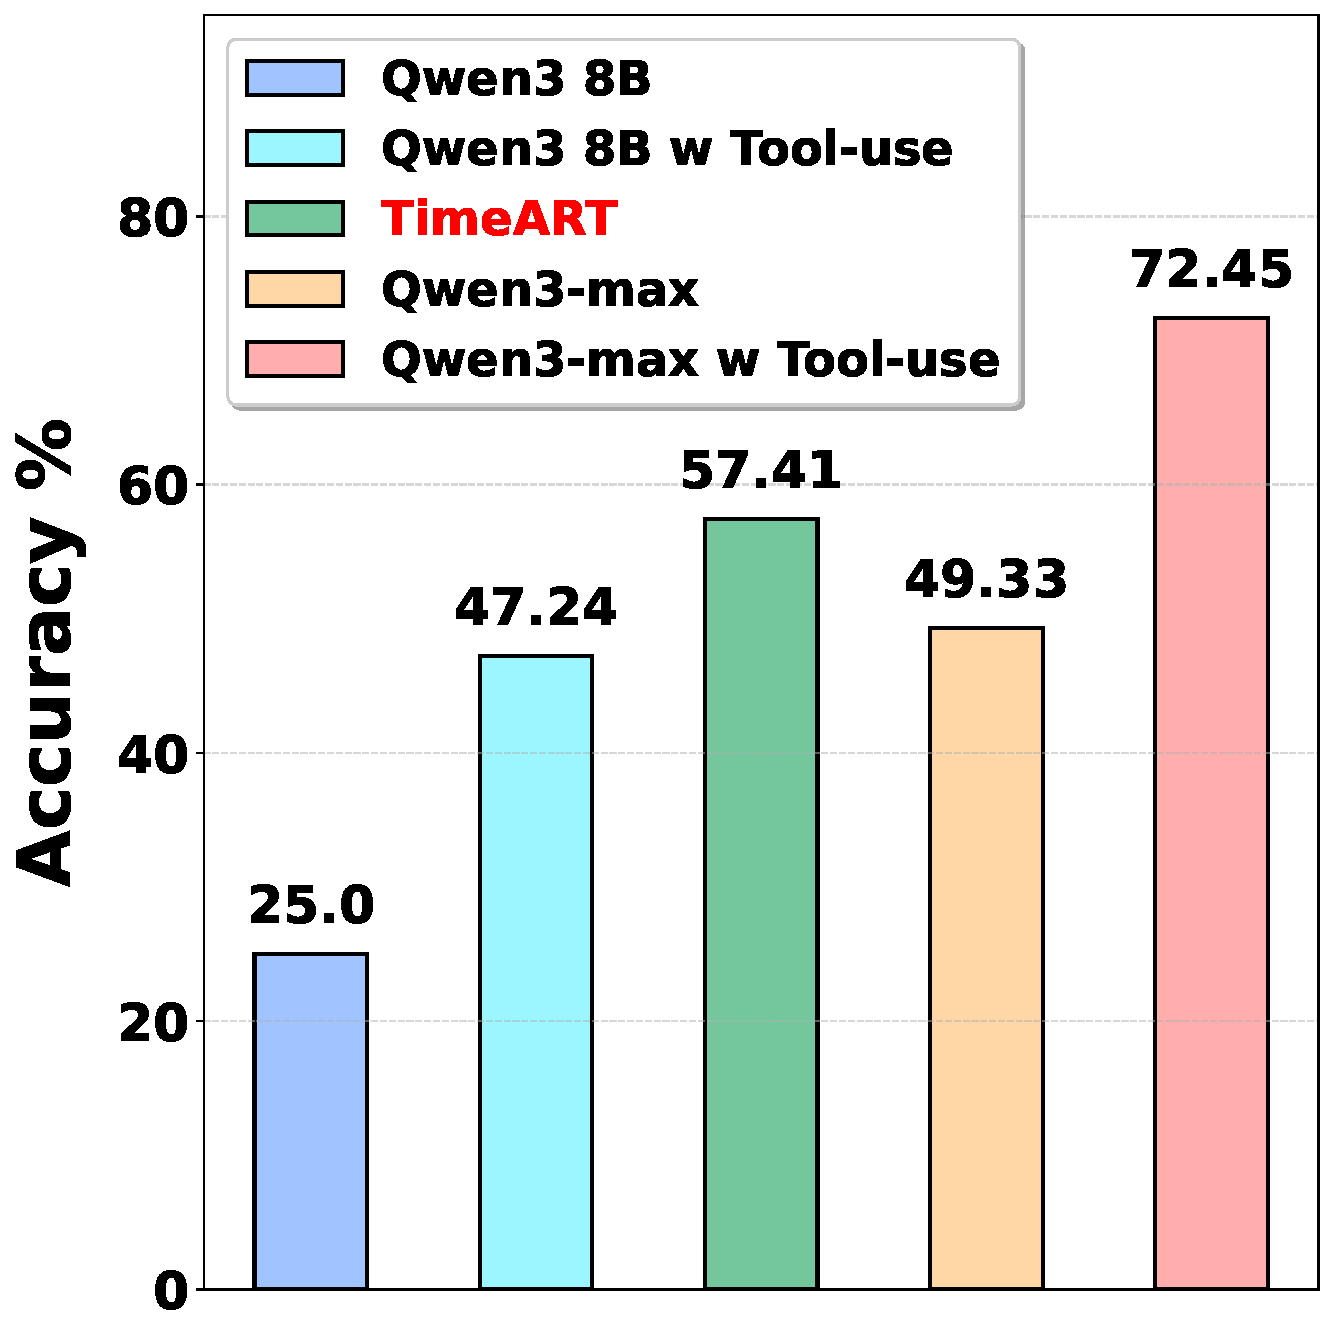
\includegraphics[width=\linewidth]{Figures/ablations-framework-estimation.pdf}}
  \end{minipage}
  \caption{Ablations on the TimeART framework.}
  \label{fig: ablations on framework}

  \vspace{-3mm}
\end{figure}


\begin{figure*}[!htbp]
  \centering
  % 第一个子图
  \begin{minipage}[b]{0.24\linewidth}
    \centering
    \subfloat[Understanding.]
    {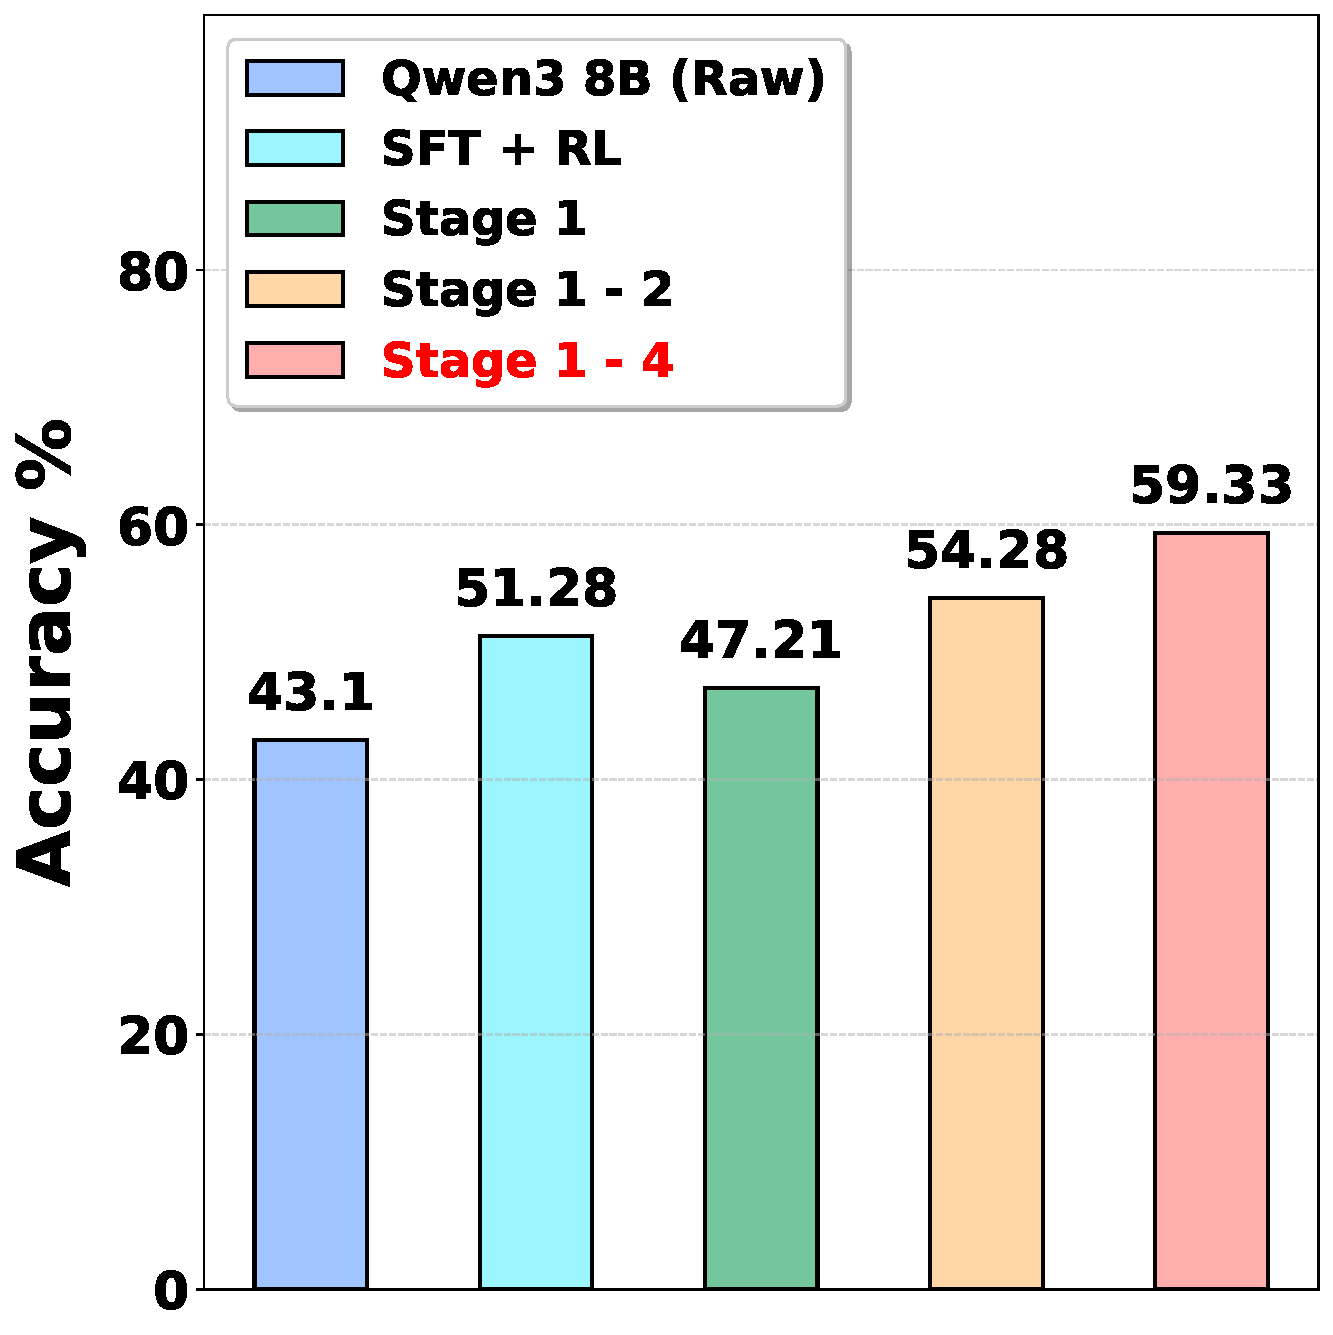
\includegraphics[width=\linewidth]{Figures/ablations-training-understanding.pdf}}
  \end{minipage}
  \hfill % 使用 fill 自动分配间距
  % 第二个子图
  \begin{minipage}[b]{0.24\linewidth}
    \centering
    \subfloat[Perception.]
    {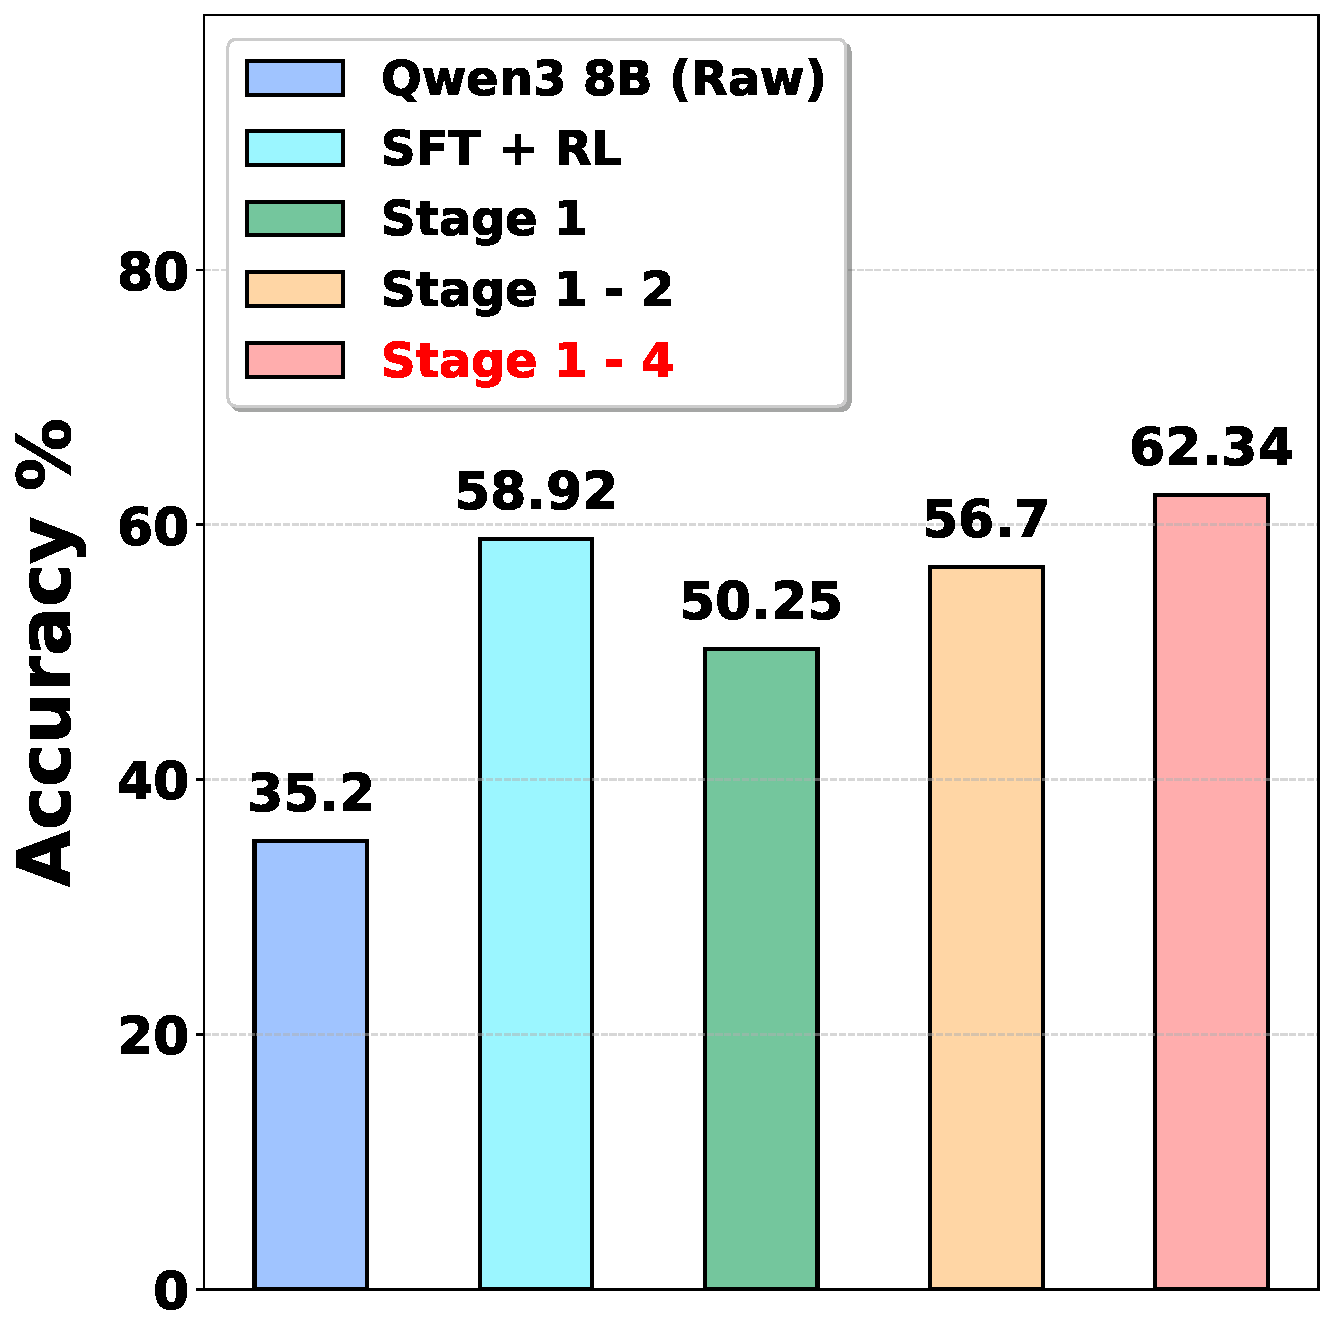
\includegraphics[width=\linewidth]{Figures/ablations-training-perception.pdf}}
  \end{minipage}
  \hfill
  % 第三个子图
  \begin{minipage}[b]{0.24\linewidth}
    \centering
    \subfloat[Reasoning.]
    {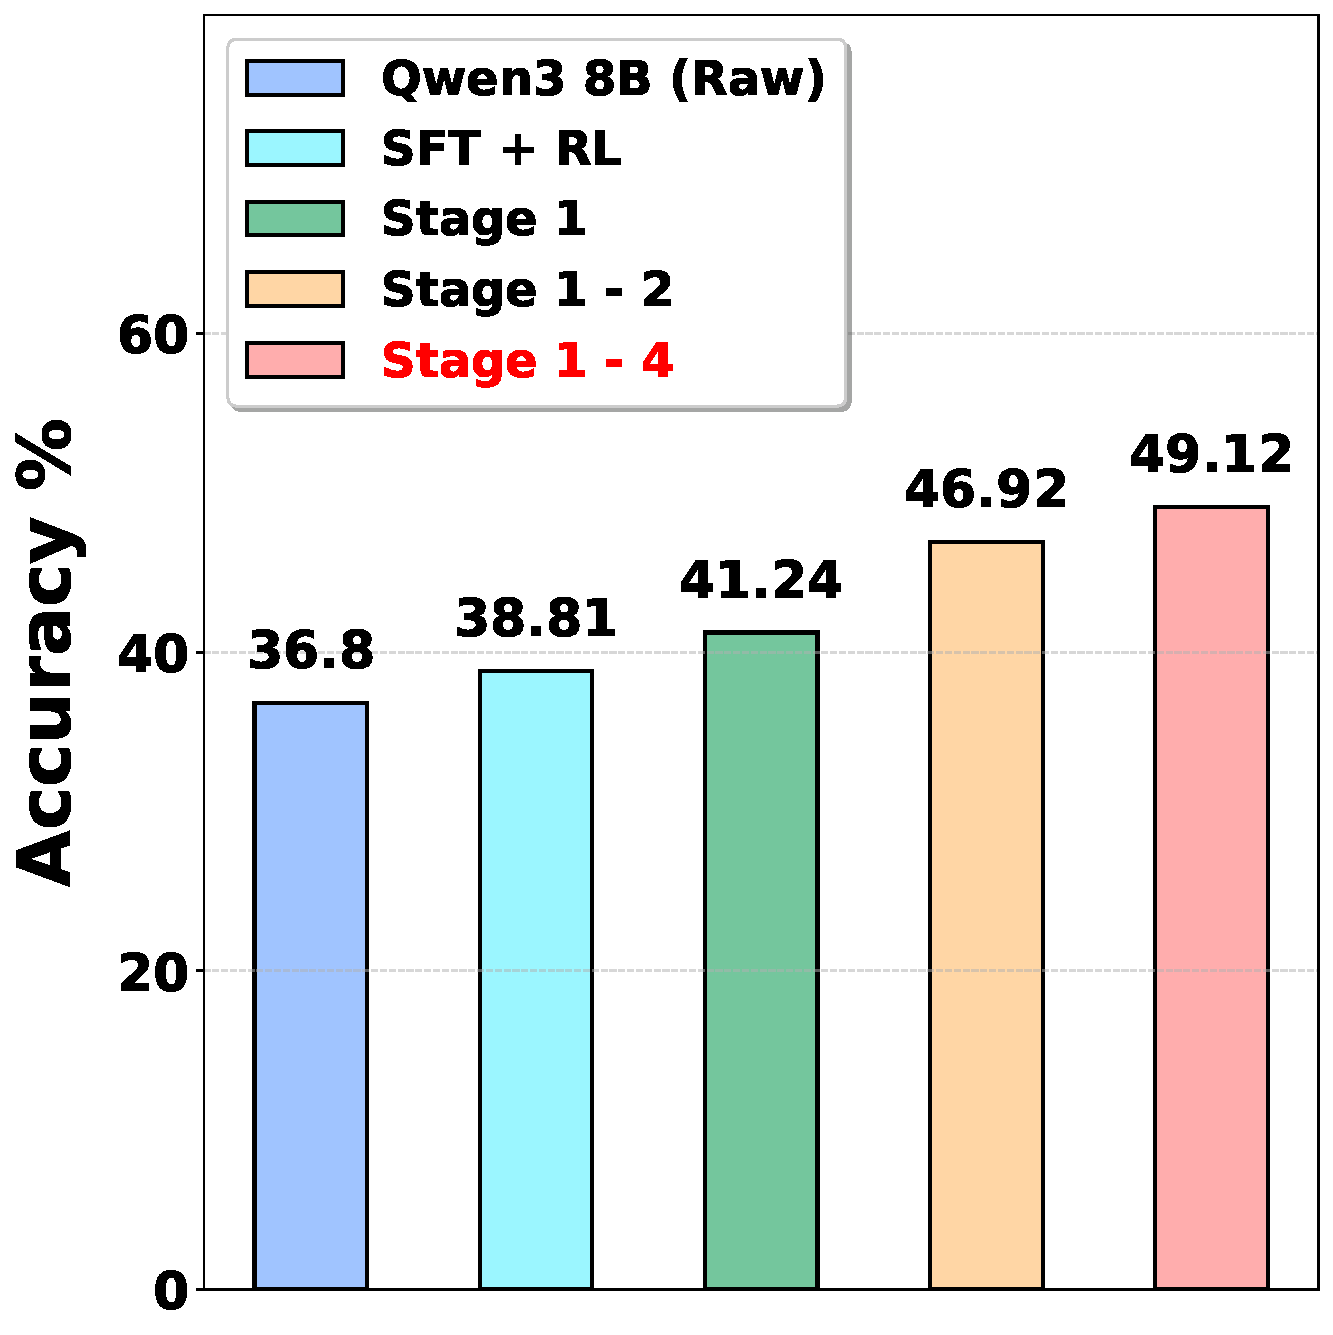
\includegraphics[width=\linewidth]{Figures/ablations-training-reasoning.pdf}}
  \end{minipage}
  \hfill
  % 第四个子图
  \begin{minipage}[b]{0.24\linewidth}
    \centering
    \subfloat[Estimation.]
    {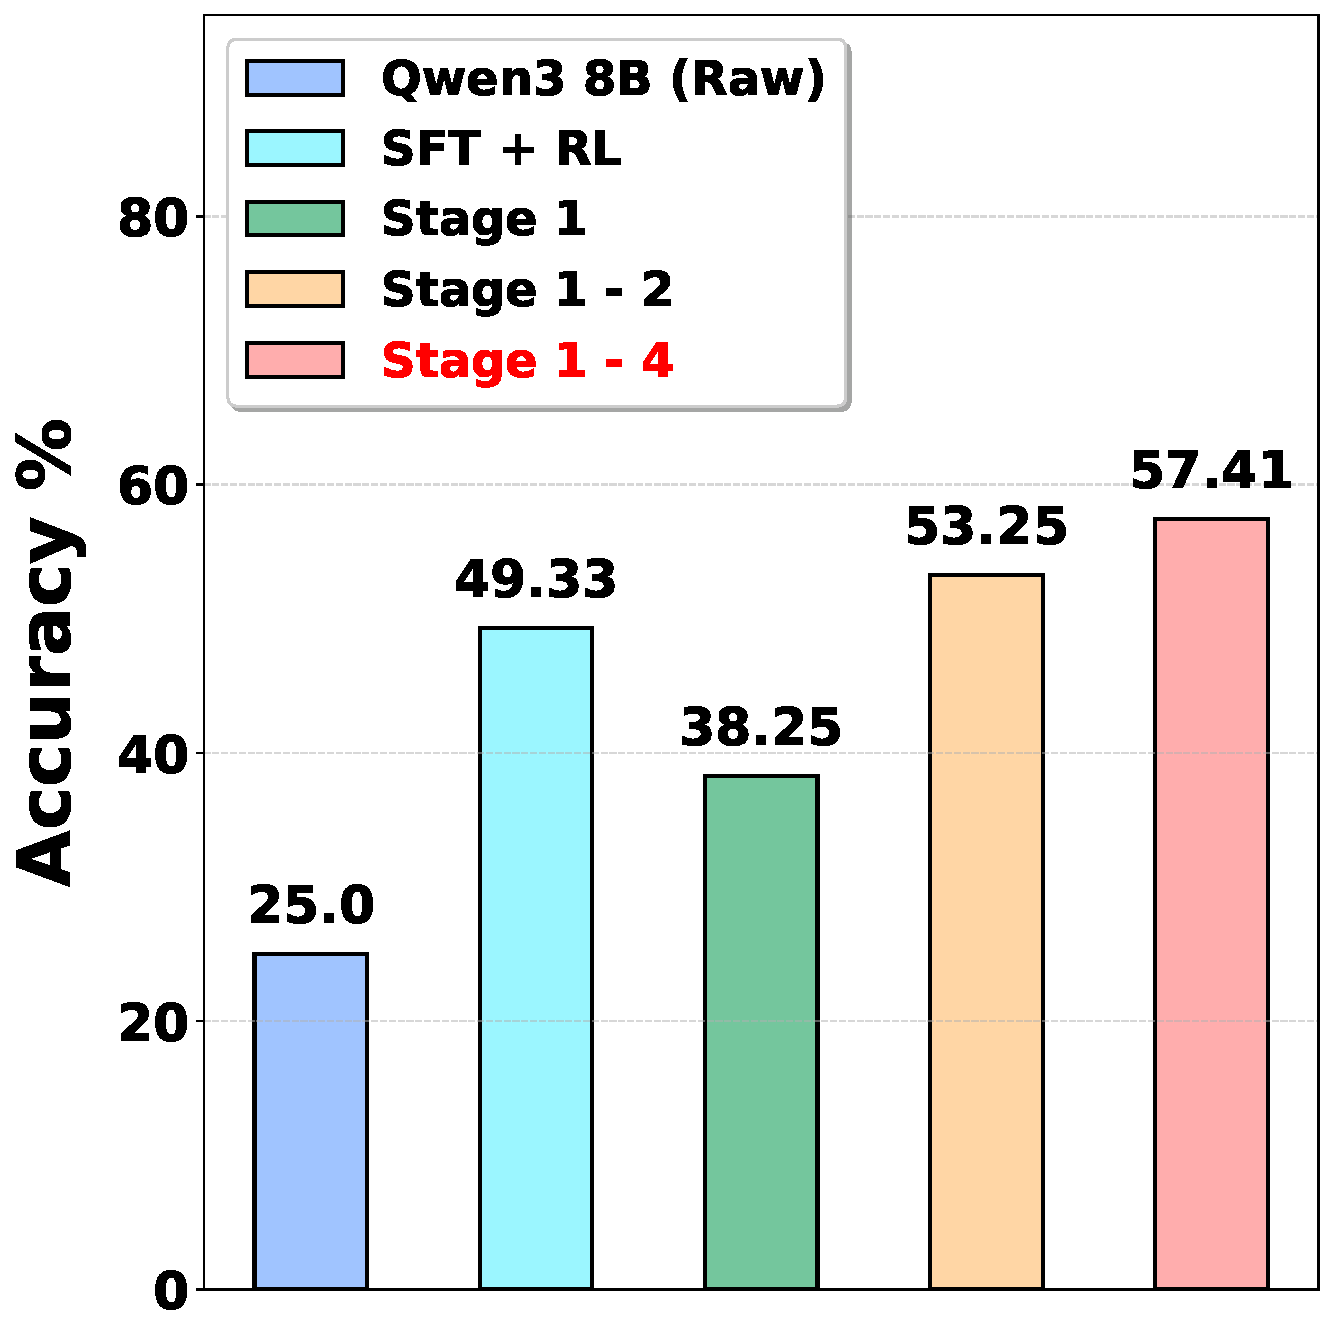
\includegraphics[width=\linewidth]{Figures/ablations-training-estimation.pdf}}
  \end{minipage}
  
  \caption{Ablations on training stages.}
  \label{fig: ablations on training}
\end{figure*}

%raw sft+rl stage1 stage1+2 all
\textbf{Ablations on training stages.} We also study on the proposed training strategy to validate its effectiveness. Since it consists of four key stages, among them, Stage 1 and Stage 2 are independent, and Stage 3 and 4 are coherent. We design the following configurations: 1) Original Qwen3 8B as a fundamental baseline; 2) Conventional (SFT + RL) training strategy used to compare with our proposed strategy; 3) Only using the Stage 1 to evalaute its effectiveness; 4) Only using the Stage 1 and 2 to validate whether the SFT (Stage 2) can further improved after Stage 1; 5) Using all the training stages (ours). 

As shown in Figure~\ref{fig: ablations on training}, the experiments are also conducted on the four categories of reasoning tasks from TimeMQA. We have the following key conclusions: 1) Stage 1 is important. We observe that the performance is consistently improved on all TSQA tasks, and on the reasoning task, its performance even outperforms conventional (SFT + RL) training process. This indicates the capability boundaries of tools are key information, and Stage 1 helps TSRMs internalize them like a world model, thus can predict the effects of specific tools in specific situations; 2) Stage 1 can help mitigate the low generalization dilemma in SFT (Stage 2). We observe that training the Qwen3 8B with only Stage 1 and 2 can outperform conventional (SFT + RL) training process in most cases. Since Stage 1 has already taught the TSRMs the tools' capability boundaries, this provides a previous knowledge preserve and makes Stage 2 beyond 


simple imitations, keeping the general tool-use principles from converging to make some conservative decisions; 3) Learning from self-reflection (Stage 3 + 4) is also vital. It is observed that training on all stages is consistently the best strategy on all TSQA tasks. These two stages replace fixed manually-designed preferences (reward models) with flexible self-reflected internal logic, thus boosting self-evolution of agents through internal logical thinking.